
\documentclass[12pt,halfline,a4paper,]{ouparticle}

% Packages I think are necessary for basic Rmarkdown functionality
\usepackage{hyperref}
\usepackage{graphicx}
\usepackage{listings}
\usepackage{xcolor}
\usepackage{fancyvrb}
\usepackage{framed}

% Link coloring
\hypersetup{breaklinks=true,
            bookmarks=true,
            pdfauthor={},
            pdftitle={Spatial Coordination Of Stomatal Patterning Between Leaf Surfaces In Amphistomatous Arabidopsis thaliana Incurs No Photosynthetic Advantage}
            }


%% To allow better options for figure placement
%\usepackage{float}

% Packages that are supposedly required by OUP sty file
\usepackage{amssymb, amsmath, geometry, amsfonts, verbatim, endnotes, setspace}

% use upquote if available, for straight quotes in verbatim environments
\IfFileExists{upquote.sty}{\usepackage{upquote}}{}

% Macros for dealing with affiliations, footnotes, etc.
\makeatletter
\def\Newlabel#1#2#3{\expandafter\gdef\csname #1@#2\endcsname{#3}}

\def\Ref#1#2{\@ifundefined{#1@#2}{???}{\csname #1@#2\endcsname}}

\newcommand*\samethanks[1][\value{footnote}]{\footnotemark[#1]}

\newcommand*\ifcounter[1]{%
  \ifcsname c@#1\endcsname
    \expandafter\@firstoftwo
  \else
    \expandafter\@secondoftwo
  \fi
}

\newcommand*\thanksbycode[1]{%
  \ifcounter{FNCT@#1}
    {\samethanks[\value{FNCT@#1}]}
    {\thanks{\Ref{FN}{#1}}\newcounter{FNCT@#1}\setcounter{FNCT@#1}{\value{footnote}}}
}

% Create labels for Addresses if the are given in Elsevier format
\Newlabel{ADR}{Colgate University}{13 Oak Drive, Hamilton, NY 13346}
\Newlabel{ADR}{University of Hawaii at Manoa}{2500 Campus Rd, Honolulu,
HI 96822}

% Create labels for Footnotes if the are given in Elsevier format
\Newlabel{FN}{1}{Equal contribution}
\Newlabel{FN}{2}{Current email address:
\href{mailto:cat@example.com}{cat@example.com}}

% Part for setting citation format package: natbib

% Part for setting citation format package: biblatex


% tightlist command for lists without linebreak
\providecommand{\tightlist}{%
  \setlength{\itemsep}{0pt}\setlength{\parskip}{0pt}}


% Pandoc citation processing
\newlength{\cslhangindent}
\setlength{\cslhangindent}{1.5em}
\newlength{\csllabelwidth}
\setlength{\csllabelwidth}{3em}
\newlength{\cslentryspacingunit} % times entry-spacing
\setlength{\cslentryspacingunit}{\parskip}
% for Pandoc 2.8 to 2.10.1
\newenvironment{cslreferences}%
  {}%
  {\par}
% For Pandoc 2.11+
\newenvironment{CSLReferences}[2] % #1 hanging-ident, #2 entry spacing
 {% don't indent paragraphs
  \setlength{\parindent}{0pt}
  % turn on hanging indent if param 1 is 1
  \ifodd #1
  \let\oldpar\par
  \def\par{\hangindent=\cslhangindent\oldpar}
  \fi
  % set entry spacing
  \setlength{\parskip}{#2\cslentryspacingunit}
 }%
 {}
\usepackage{calc}
\newcommand{\CSLBlock}[1]{#1\hfill\break}
\newcommand{\CSLLeftMargin}[1]{\parbox[t]{\csllabelwidth}{#1}}
\newcommand{\CSLRightInline}[1]{\parbox[t]{\linewidth - \csllabelwidth}{#1}\break}
\newcommand{\CSLIndent}[1]{\hspace{\cslhangindent}#1}

\usepackage[nomarkers,tablesfirst]{endfloat}
\usepackage{lineno}
\linenumbers
\usepackage{hyperref}
\renewcommand{\figureautorefname}{Fig.}
\usepackage{booktabs}

\begin{document}

\title{Spatial Coordination Of Stomatal Patterning Between Leaf Surfaces
In Amphistomatous \emph{Arabidopsis thaliana} Incurs No Photosynthetic
Advantage}

\author{%
%
% Code for old style authors field
%
% Add \and if both authors and author
%
%
% Code for new (elsevier) style author field
\name{Jacob L. Watts}
\address{\Ref{ADR}{Colgate University}}
%
\email{\href{mailto:jwatts@colgate.edu}{jwatts@colgate.edu}}%
\thanks{Corresponding author; Email: \href{mailto:jwatts@colgate.edu}{jwatts@colgate.edu}}%
%
%
\and
\name{Graham Dow}
\address{\Ref{ADR}{ETH}}
%
\email{\href{mailto:graham.dow@usys.ethz.ch}{graham.dow@usys.ethz.ch}}%
%
%
%
\and
\name{Thomas N. Buckley}
\address{\Ref{ADR}{University of California Davis}}
%
\email{\href{mailto:tnbuckley@ucdavis.edu}{tnbuckley@ucdavis.edu}}%
%
%
\thanksbycode{1}
%
\and
\name{Christopher D. Muir}
\address{\Ref{ADR}{University of Hawaii at Manoa}}
%
\email{\href{mailto:cdmuir@hawaii.edu}{cdmuir@hawaii.edu}}%
%
%
\thanksbycode{1}
%
%
}

\abstract{This is the abstract.

It consists of two paragraphs.}

\date{\today}

\keywords{amphistomy; Arabidopsis thaliana; CO\(_2\) diffusion; finite
element method; optimality; photosynthesis; stomata}

\maketitle



\hypertarget{introduction}{%
\section{Introduction}\label{introduction}}

Stomatal anatomy (e.g.~size, density, distribution, and patterning) and
movement regulate gas exchange during photosynthesis, namely CO\(_2\)
assimilation and water loss through transpiration. Since waxy cuticles
are mostly impermeable to CO\(_2\) and H\(_2\)O, stomata are the primary
entry points through which gas exchange occurs despite making up a small
percentage of the leaf area
(\protect\hyperlink{ref-lange_responses_1971}{Lange et al. 1971}).
Stomata consist of two guard cells which open and close upon changes in
turgor pressure or hormonal cues
(\protect\hyperlink{ref-mcadam_linking_2016}{McAdam and Brodribb 2016}).
The stomatal pore leads to an internal space known as the substomatal
cavity where gases contact the mesophyll. Once in the mesophyll,
CO\(_2\) diffuses throughout a network of intercellular air space (IAS)
and into mesophyll cells where CO\(_2\) assimilation (\(A\)) occurs
within the chloroplasts (\protect\hyperlink{ref-lee_diffusion_1964}{Lee
and Gates 1964}). Stomatal conductance and transpiration are determined
by numerous environmental and anatomical parameters such as vapor
pressure deficit (VPD), irradiance, temperature, wind speed, leaf water
potential, IAS geometry, mesophyll cell anatomy, and stomatal anatomy.

Many successful predictions about stomata and other leaf traits can be
made by hypothesizing that natural selection should optimizes CO\(_2\)
gain per unit of water loss
(\protect\hyperlink{ref-cowan_stomatal_1977}{Cowan and Farquhar 1977};
\protect\hyperlink{ref-buckley_optimal_2017}{Buckley, Sack, and Farquhar
2017}; \protect\hyperlink{ref-sperry_predicting_2017}{Sperry et al.
2017}). However, stomatal anatomy may be partially constrained by
physical and developments limits on phenotypic expression
(\protect\hyperlink{ref-croxdale_stomatal_2000}{Croxdale 2000};
\protect\hyperlink{ref-harrison_influence_2020}{Harrison et al. 2020};
\protect\hyperlink{ref-muir_how_2023}{Christopher D. Muir et al. 2023}).
Sometimes optimization leads to similar phenotypes across many disparate
species. For example, almost all stomata follow the one cell spacing
rule to maintain proper stomatal functioning
(\protect\hyperlink{ref-geisler_oriented_2000}{Geisler, Nadeau, and Sack
2000}; \protect\hyperlink{ref-dow_physiological_2014}{Dow, Berry, and
Bergmann 2014}); however some species (notably in \emph{Begonia}) appear
to benefit from overlapping vapor shells caused by stomatal clustering
(\protect\hyperlink{ref-yi_gan_stomatal_2010}{Yi Gan et al. 2010};
\protect\hyperlink{ref-lehmann_effects_2015}{Lehmann and Or 2015};
\protect\hyperlink{ref-papanatsiou_stomatal_2017}{Papanatsiou, Amtmann,
and Blatt 2017}). Stomatal traits also vary adaptively in different
environments. Stomatal density positively co-varies with irradiance
during leaf development and negatively co-varies with CO\(_2\)
concentration (\protect\hyperlink{ref-gay_influence_1975}{Gay and Hurd
1975}; \protect\hyperlink{ref-schoch_dependence_1980}{Schoch, Zinsou,
and Sibi 1980}; \protect\hyperlink{ref-woodward_stomatal_1987}{Woodward
1987}; \protect\hyperlink{ref-royer_stomatal_2001}{Royer 2001}),
consistent with optimality predictions. Stomatal size is jointly
controlled by genome size, light, and stomatal density
(\protect\hyperlink{ref-jordan_environmental_2015}{Jordan et al. 2015}).
Size positively co-varies with genome size
(\protect\hyperlink{ref-roddy_scaling_2020}{Roddy et al. 2020}) and
negatively co-varies with stomatal density
(\protect\hyperlink{ref-camargo_density_2011}{Camargo and Marenco
2011}). Total stomatal area (size \(\times\) density) is optimized for
operational conductance (\(gs_\text{s,op}\)) rather than maximum
conductance (\(gs_\text{s,max}\)) such that stomatal apertures are most
responsive to changes in the environment at their operational aperture
(\protect\hyperlink{ref-franks_physiological_2012}{Franks et al. 2012};
\protect\hyperlink{ref-liu_scaling_2021}{Liu et al. 2021}). Stomatal
aperture can compensate for maladaptive stomatal densities to an extent
(\protect\hyperlink{ref-bussis_stomatal_2006}{Büssis et al. 2006}), but
stomatal density and size ultimately determine a leaf's theoretical
\(gs_\text{s,max}\)
(\protect\hyperlink{ref-sack_developmental_2016}{Sack and Buckley
2016}), which is proportional to \(gs_\text{s,op}\)
(\protect\hyperlink{ref-murray_consistent_2020}{Murray et al. 2020}).
Additionally, low stomatal densities lead to irregular and insufficient
CO\(_2\) supply and reduced photosynthetic efficiency in areas far from
stomata (\protect\hyperlink{ref-pieruschka_lateral_2006}{Roland
Pieruschka et al. 2006};
\protect\hyperlink{ref-morison_lateral_2005}{Morison et al. 2005}),
while high stomatal densities can reduce water use efficiency (WUE)
(\protect\hyperlink{ref-bussis_stomatal_2006}{Büssis et al. 2006}) and
incur excessive metabolic costs
(\protect\hyperlink{ref-deans_optimization_2020}{Deans et al. 2020}). In
most species, stomata occur on the abaxial (usually lower) leaf surface;
but amphistomy, the occurrence of stomata on both abaxial and adaxial
leaf surfaces, is also prevalent in high light environments with
constant or intermittent access to sufficient water
(\protect\hyperlink{ref-mott_adaptive_1982}{Mott, Gibson, and O'Leary
1982}; \protect\hyperlink{ref-jordan_using_2014}{Jordan, Carpenter, and
Brodribb 2014}; \protect\hyperlink{ref-muir_light_2018}{Christopher D.
Muir 2018}; \protect\hyperlink{ref-drake_two_2019}{Drake et al. 2019};
\protect\hyperlink{ref-muir_is_2019}{Christopher D. Muir 2019}).
Amphistomy effectively halves the CO\(_2\) diffusion path length and
boundary layer resistance by doubling boundary layer conductance
(\protect\hyperlink{ref-parkhurst_adaptive_1978}{Parkhurst 1978};
\protect\hyperlink{ref-harrison_influence_2020}{Harrison et al. 2020};
\protect\hyperlink{ref-mott_amphistomy_1991}{Mott and Michaelson 1991}).
Historically, stomatal patterning in dicot angiosperms was thought to be
random with an exclusionary distance surrounding each stomate
(\protect\hyperlink{ref-sachs_developmental_1974}{Sachs 1974}); however,
the developmental controls of stomatal patterning are poorly understood
and likely more complex than random development along the leaf surface.
Croxdale (\protect\hyperlink{ref-croxdale_stomatal_2000}{2000}){]}
reviews three developmental theories which attempt to explain stomatal
patterning in angiosperms: inhibition, cell lineage, and cell cycle,
ultimately arguing for a cell cycle based control of stomatal
patterning.

The patterning and spacing of stomata on the leaf affects photosynthesis
in \(C_3\) leaves by altering the CO\(_2\) diffusion path length from
stomata to sites of carboxylation in the mesophyll. Maximum
photosynthetic rate (\(A_\text{max}\)) in \(C_3\) plants is generally
co-limited by biochemistry and diffusion, but modulated by light
availability
(\protect\hyperlink{ref-parkhurst_intercellular_1990}{Parkhurst and Mott
1990}; \protect\hyperlink{ref-manter_ci_2004}{Manter 2004};
\protect\hyperlink{ref-carriqui_diffusional_2015}{Carriquí et al.
2015}). Low light decreasing CO\(_2\) demand by limiting electron
transport rate, leading to relatively high internal CO\(_2\)
concentration (\(C_\text{i}\)) and low \(A_\text{max}\)
(\protect\hyperlink{ref-kaiser_metabolic_2016}{Kaiser et al. 2016}). In
contrast, well hydrated leaves with open stomata in high light,
photosynthesis is often limited by CO\(_2\) supply as resistances from
the boundary layer, stomatal pore, and mesophyll can result in
insufficient CO\(C_2\) supply at the chloroplast to maxmimize
photosynthesis
(\protect\hyperlink{ref-farquhar_biochemical_1980}{Farquhar, Caemmerer,
and Berry 1980}; \protect\hyperlink{ref-lehmeier_cell_2017}{Lehmeier et
al. 2017}). In this study, we focus primarily on how stomatal patterning
affects diffusion, ignoring boundary layer and mesophyll resistances.

To maximize CO\(_2\) supply from the stomatal pore to chloroplasts,
stomata should be uniformly distributed in an equilateral triangular
grid on the leaf surface so as to minimize stomatal number and CO\(_2\)
diffusion path length
(\protect\hyperlink{ref-parkhurst_diffusion_1994}{Parkhurst 1994}). As
the diffusion rate of CO\(_2\) though liquid is approximately
\(10^4\times\) slower than CO\(_2\) diffusion through air, mesophyll
resistance is generally thought to be primarily limited by liquid
diffusion (\protect\hyperlink{ref-aalto_three-dimensional_2002}{Aalto
and Juurola 2002}; \protect\hyperlink{ref-evans_resistances_2009}{J. R.
Evans et al. 2009}), but diffusion through the IAS has also been shown
to be a rate limiting process because the tortuous, disjunct nature of
the IAS can greatly increase diffusion path lengths
(\protect\hyperlink{ref-harwood_understanding_2021}{Harwood,
Théroux‐Rancourt, and Barbour 2021}). Additionally, tortuosity is higher
in horizontal directions (parallel to leaf surface) than vertical
directions (perpendicular to leaf surface) because of the cylindrical
shape and vertical arrangement of pallisade mesophyll cells
(\protect\hyperlink{ref-earles_beyond_2018}{Earles et al. 2018};
\protect\hyperlink{ref-harwood_understanding_2021}{Harwood,
Théroux‐Rancourt, and Barbour 2021}). However, the ratio of lateral to
vertical diffusion rate is still largely unknown
(\protect\hyperlink{ref-morison_lateral_2005}{Morison et al. 2005};
\protect\hyperlink{ref-pieruschka_lateral_2005}{R. Pieruschka 2005};
\protect\hyperlink{ref-pieruschka_lateral_2006}{Roland Pieruschka et al.
2006}). Depending on the thickness of the leaf, porosity of the leaf
mesophyll, tortuosity of the IAS, and lateral to vertical diffusion rate
ratio, minimizing diffusion path length for CO\(_2\) via optimally
distributed stomata may yield significant increases in CO\(_2\) supply
for photosynthesis and higher \(A_\text{max}\).

We hypothesized that natural selection will favor stomatal patterning
and distribution to minimize the diffusion path length. In
amphistomatous leaves, this would be accomplished by 1) a uniform
distribution of stomata on both abaxial and adaxial leaf surfaces and 2)
coordinated stomatal spacing on each surface that offsets the position
of stomata (\autoref{fig:ideal-amphi-grid}). Coordination between leaf
surfaces is defined in this study as the occurrence of stomata in areas
farthest from stomata on the opposite leaf surface. Additionally,
because CO\(_2\) is more limiting for photosynthesis under high light,
we hypothesize that in high light 3) there should be more stomata, and
4) stomata should be more uniformly distributed than in low light.
Finally, as stomatal densities are selected for optimal operational
aperture, we hypothesize that 5) stomatal length will be positively
correlated with the area of the leaf surface to which it is closest. We
refer to this as the `stomatal zone', the leaf area surrounding a focal
stomate closest to that stomate and therefore the zone it supplies with
CO\(_2\)). This way, each stomate can be optimally sized relative to the
mesophyll volume it supplies.

\begin{figure}[ht]
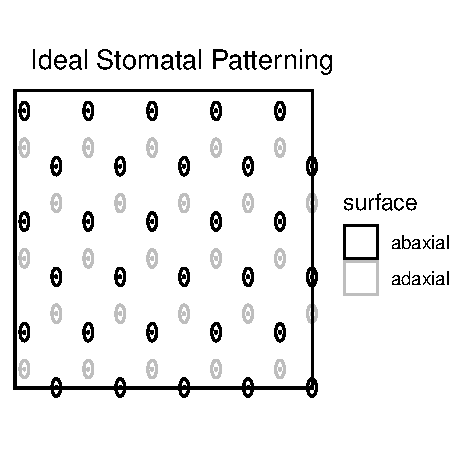
\includegraphics[width = \textwidth]{figures/ideal-amphi-grid.pdf}
\caption{Idealized amphistomatous stomatal grid with uniform stomatal patterning and perfect abaxial-adaxial coordination.}
\label{fig:ideal-amphi-grid}
\end{figure}

To test these hypotheses, we grew the model plant \emph{Arabidopsis
thaliana} in high, medium, and low light and measured stomatal density,
size, and patterning on both leaf surfaces, and spatial coordination
between them. We use Voronoi tessellation techniques to calculate
stomatal zones. We also used a 2-D porous medium approximation of
CO\(_2\) diffusion and photosynthesis to predict the photosynthetic
advantage of optimal versus suboptimal coordination in stomatal
coordination between surfaces. Specifically, we predicted that traits
which affect diffusion path length (leaf thickness, stomatal density,
leaf porosity, lateral-vertical diffusion rate ratio), diffusion rate
(temperature, pressure), and CO\(_2\) demand (Rubisco concentration,
light) would modulate the advantage of optimal stomatal arrangement
following the relationships outlined in \autoref{tab:hypotheses}. Here,
we integrate over reasonable parameter space to determine the
ecophysiological context most likely to favor stomatal spatial
coordination in amphistomatous leaves.

\begin{table}[ht]
\centering
\begin{tabular}{ll}
  \hline
trait & relationship \\ 
  \hline
leaf thickness & + \\ 
  stomatal density & - \\ 
  leaf porosity & - \\ 
  lat.-vert. diffusion ratio & - \\ 
  temperature & - \\ 
  pressure & - \\ 
  Rubisco concentration & + \\ 
  light & + \\ 
   \hline
\end{tabular}
\caption{A summary of the hypothesized relationships between leaf traits and environmental conditions and photosynthetic advantage of stomatal spatial coordination in amphistomatous leaves.} 
\label{tab:hypotheses}
\end{table}

\hypertarget{materials-and-methods}{%
\section{Materials and methods}\label{materials-and-methods}}

\hypertarget{data-preparation}{%
\subsection{Data Preparation}\label{data-preparation}}

{[}CDM: Graham Dow provided these images. We'll need to add him as a
co-author and ask him to write methods on image acquisition.{]}

\emph{Arabidopsis thaliana} plants were grown in three different light
environments: low light (PAR = 50
\(\mu \text{mol}~\text{m}^{-2}~\text{s}^{-1}\)), medium light (100
\(\mu \text{mol}~\text{m}^{-2}~\text{s}^{-1}\)), and high light (200
\(\mu \text{mol}~\text{m}^{-2}~\text{s}^{-1}\)). PAR stands for
photosynthetically active radiation. Once leaves were mature, we
captured images of the abaxial and adaxial leaf surfaces using XXX. We
captured 132 images in total, making 66 abaxial-adaxial image pairs. We
measured stomatal position and size using ImageJ
(\protect\hyperlink{ref-schneider_nih_2012}{Schneider, Rasband, and
Eliceiri 2012}).

\hypertarget{single-surface-analyses}{%
\subsection{Single surface analyses}\label{single-surface-analyses}}

We tested whether stomata are non-randomly distributed by comparing the
observed stomatal patterning to a random uniform pattern. For each leaf
surface image with \(n\) stomata we generated \(10^3\) synthetic
surfaces with \(n\) stomata uniformly randomly distributed on the
surface. For each sample image, we compared the observed Nearest
Neighbor Index (\(\mathrm{NNI}\)) to the null distribution of
\(\mathrm{NNI}\) values calculated from the synthetic data set.
\(\mathrm{NNI}\) is the ratio of observed mean distance
(\(\overline{D}_O\)) to the expected mean distance (\(\overline{D}_E\))
where \(\overline{D}_E\) is:

\begin{equation}\label{eq:emd}
  \overline{D}_E = \frac{0.5}{\sqrt{A_\text{leaf} / n_\text{stomata}}}.
\end{equation}

\noindent \(A_\text{leaf}\) is leaf area visible in the sampled field
and \(n_\text{stomata}\) the number of stomata. \(\overline{D}_E\) is
the theoretical average distance to the nearest neighbor of each stomate
if stomata were uniformly randomly distributed
(\protect\hyperlink{ref-clark_distance_1954}{Clark and Evans 1954}).
\(\overline{D}_O\) calculated for each synthetic data set is:

\begin{equation}\label{eq:omd}
  \overline{D}_O = \frac{\sum_{i=1}^{n_\text{stomata}}d_i}{n_\text{stomata}},
\end{equation}

\noindent where \(d_i\) is the distance between \(\text{stomate}_i\) and
its nearest neighbor. We calculated \(\mathrm{NNI}\) using the \emph{R}
package \textbf{spatialEco} version 2.0.1
(\protect\hyperlink{ref-evans_spatialeco_2023}{J. S. Evans and Murphy
2023}). The observed stomatal distribution is dispersed relative to a
uniform random distribution if the observed \(NNI\) is greater than 95\%
of the synthetic \(\mathrm{NNI}\) values (one-tailed test). We adjusted
\(P\)-values to account for multiple comparisons using the
Benjamini-Hochberg
(\protect\hyperlink{ref-benjamini_controlling_1995}{\textbf{benjamini\_controlling\_1995?}})
false discovery rate procedure implemented in the \emph{R} package
\textbf{multtest} version 2.56.0
(\protect\hyperlink{ref-pollard_multiple_2005}{\textbf{pollard\_multiple\_2005?}}).

For each sample image, we also simulated \(10^3\) synthetic data with
\(n\) stomata ideally dispersed in an equilateral triangular grid. For
these grids, we integrated over plausible stomatal densities and then
conditioned on stomatal grids with exactly \(n\) stomata. The simulated
stomatal count was drawn from a Poisson distribution with the mean
parameter \(\lambda\) drawn from a Gamma distribution with shape \(n\)
and scale 1 \(\lambda \sim \Gamma(n, 1)\). \(\Gamma(n, 1)\) is the
posterior distribution of \(\lambda\) with a flat prior distribution.
This allows us to integrate over uncertainty in the stomatal density
from the sample image.

We developed a dispersion index \(\mathrm{DI}\) to quantify how close
observed stomatal distributions are to random uniform versus maximally
dispered in an equilateral triangular grid. \(\mathrm{DI}\) varies from
zero to one, where zero is uniformly random and one is ideally
dispersed:

\begin{equation}\label{eq:disp}
  \mathrm{DI} = \frac{\mathrm{NNI} - \text{median}(\mathrm{NNI_{random}})}{\text{median}(\mathrm{NNI_{uniform}}) - \text{median}(\mathrm{NNI_{random}})}
\end{equation}

\noindent \(\mathrm{NNI}\) is calculated for each sample image as
described above; \(\text{median}(\mathrm{NNI_{random}})\) and
\(\text{median}(\mathrm{NNI_{uniform}})\) are calculated from the
synthetic data specific to each sample image as described above. We
tested whether light treatment affects \(\mathrm{DI}\) and stomatla
density (\(D_S\)) using analysis of variance (ANOVA).

Finally, we examined the relationship between stomatal zone area and
stomatal length using a Bayesian generalized non-linear multilevel model
fit with the \emph{R} package \textbf{brms} version 2.15.0
(\protect\hyperlink{ref-burkner_brms_2017}{Bürkner 2017},
\protect\hyperlink{ref-burkner_advanced_2018}{2018}) and \emph{Stan}
version 2.27.0
(\protect\hyperlink{ref-stan_development_team_stan_2023}{\textbf{stan\_development\_team\_stan\_2023?}}).
Stomatal zone area was calculated using Voronoi tessellation
(e.g.~\autoref{fig:tessellation-example}). The stomatal zone area,
\(S_\text{area}\), is the region of the leaf surface whose distance to
stomate, \(S\), is less than the distance to any other stomate, \(S\).
Stomatal length was measured in ImageJ
(\protect\hyperlink{ref-schneider_nih_2012}{Schneider, Rasband, and
Eliceiri 2012}).

\begin{figure}[ht]
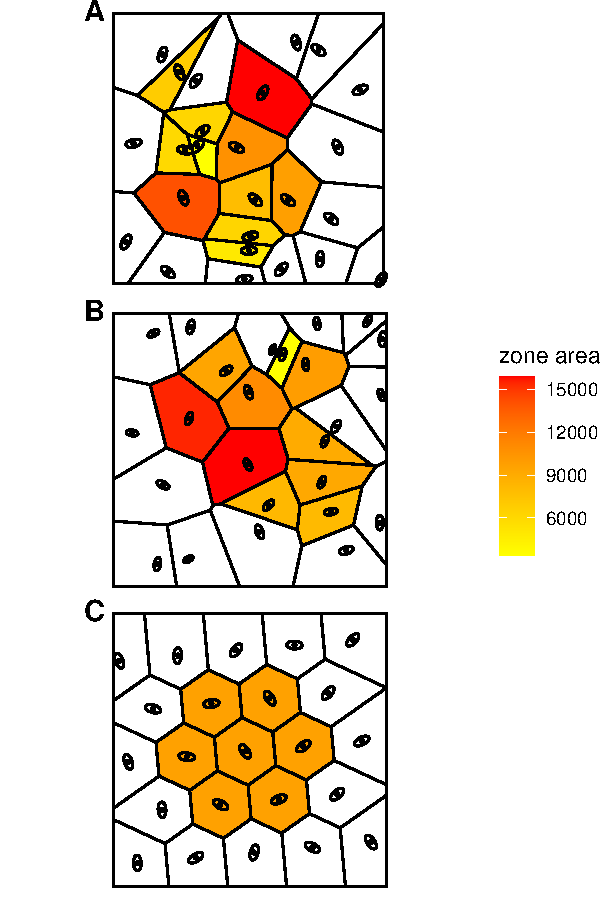
\includegraphics[width = \textwidth]{figures/tessellation-example.pdf}
\caption{Examples of synthetic and real leaf surfaces.  A) Uniform random synthetic leaf surface; B) Example of real leaf surface; C) Regularly distributed synthetic leaf surface. The zone defined by each stomate was calculated with voronoi tessellation and correlated with stomatal length in real leaves.}
\label{fig:tessellation-example}
\end{figure}

\hypertarget{paired-abaxial-and-adaxial-surface-analysis}{%
\subsection{Paired Abaxial and Adaxial Surface
Analysis}\label{paired-abaxial-and-adaxial-surface-analysis}}

To test whether the position of ab- and adaxial stomata are coordinated
we compared the observed distribution to a null distribution where the
positions on each surface are random. For each pair of surfaces
(observed or synthetic) we calculated the distance squared between each
pixel to the nearest stomatal centroid with the \emph{R} package
\textbf{raster} version 3.6.26. We refer to this as the `nearest
stomatal distance' or NSD. Then we calculated the pixel-wise Pearson
correlation coefficient. If stomatal positions on each surface are
coordinated to minimize the distance between mesophyll and the nearest
stomate, then we expect a negative correlation. A pixel that is far from
a stomate on one surface should be near a stomate on the other surface
(\autoref{fig:ideal-amphi-grid}). We generated a null distribution of
the correlation coefficient by simulating \(10^3\) synthetic data sets
for each observed pair. For each synthetic data set, we simulated
stomatal position using a random uniform distribution, as described
above, matching the number of stomata on abaxial and adaxial leaf
surfaces. Stomatal positions on each surface are coordinated if the
correlation coefficient is greater than 95\% of the synthetic
correlation values (one-tailed test).

\hypertarget{modeling-photosynthesis}{%
\subsection{Modeling Photosynthesis}\label{modeling-photosynthesis}}

We modeled photosynthesis CO\(_2\) assimilation rate using a
spatially-explicit two-dimensional reaction diffusion model using a
porous medium approximation
(\protect\hyperlink{ref-parkhurst_intercellular_1994}{\textbf{parkhurst\_intercellular\_1994?}})
using the finite element method (FEM) following
(\protect\hyperlink{ref-earles_excess_2017}{\textbf{earles\_excess\_2017?}}).
Consider a two-dimensional leaf where stomata occur on each surface in a
regular sequence with interstomatal distance \(U\). The main outcome we
assessed is the advantage of offsetting the position of stomata on each
surface compared to have stomata on the same \(x\) position on each
surface. With these assumptions, by symmetry, we only need to model two
stomata, one abaxial and one adaxial, from \(x = 0\) to \(x = U/2\) and
from the adaxial surface at \(y = 0\) to the abaxial surface at
\(y = L\), the leaf thickness. We arbitrarily set the adaxial stomate at
\(x = 0\) and toggled the abaxial stomata position between \(x = U/2\)
(offset) or \(x = 0\) (below adaxial stomate). The `coordination
advantage' of offset stomatal position on each surface is the
photosynthetic rate of the leaf with offset stomata compared to that
with stomata aligned in the same \(x\) position:

\begin{equation} \label{eq:coordination_advantage}
  \text{coordination advantage} = \frac{A_\text{offset}}{A_\text{aligned}}
\end{equation}

We modeled the coordination advantage over a range of leaf thicknesses,
stomatal densities, photosynthetic capacities, and light environments to
understand when offsetting stomatal position on each surface might
deliver a significant photosynthetic advantage
(\autoref{tab:model_var}). The complete model description is available
in the Supporting Information.

\begin{table}

\caption{\label{tab:model_var}The parameter range of model variables tested for their effect on coordination advantage (\autoref{eq:coordination_advantage}) using a 2-D porous medium approximation. We used regularly spaced values within each range and simulated across all combinations. Here we converted model units to more conventional units (e.g. m to $\mu$m). $I_0$: PPFD incident on the leaf surface; $\varphi_\text{pal}$: Fraction of intercellular airspace (aka porosity), palisade; $T_\text{leaf}$: Leaf thickness; $U$: Interstomatal distance}
\centering
\begin{tabular}[t]{lll}
\toprule
Variable & Parameter range & Units\\
\midrule
$I_0$ & $50-1000$ & $\mu$mol m$^{-2}$ s$^{-1}$\\
$\varphi_\text{pal}$ & $0.1-0.3$ & m$^3$ airspace m$^{-3}$ leaf\\
$T_\text{leaf}$ & $101-501$ & $\mu$m\\
$U$ & $17-169$ & $\mu$m\\
\bottomrule
\end{tabular}
\end{table}

\hypertarget{results}{%
\section{Results}\label{results}}

Stomatal density of \emph{Arabidopsis thaliana} the 132 leaf surfaces
measured range from 12 to 93 (units) with high light leaves ranging from
93 to 55 (units), medium light from 15 to 35 (units), and low light from
12 to 42 (units). Stomatal density varies among light treatments (ANOVA,
\(F_{2,126} = 681, P = 2.88 \times 10^{-68}\)) because the density is
much greater in the high light treatment (\autoref{fig:density}).
Density is consistently greater on abaxial leaf surfaces across all
light treatments (ANOVA, \(F_{1,126} = 44.2, P = 8.21 \times 10^{-10}\);
\autoref{fig:density}). There is no evidence for an interaction between
light treatment and surface (ANOVA,
\(F_{2,126} = 2.75 \times 10^{-2}, P = 0.973\)). Leaves are
amphistomatous with a mean stomatal density ratio of 0.45.

\begin{figure}[ht]
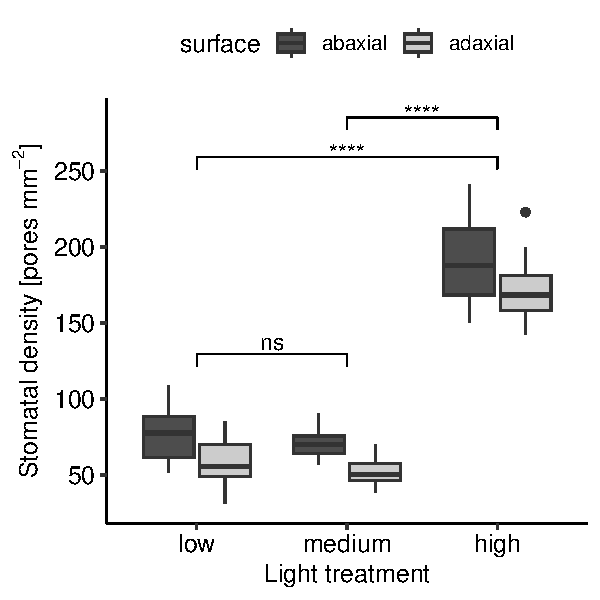
\includegraphics[width = \textwidth]{figures/density.pdf}
\caption{Stomatal density is higher in \textit{A. thaliana} plants grown under high light conditions. We determined statistical significance between light treatments using Tukey post-hoc tests. $^*~0.05 > P \ge 0.01; ^{**}~0.01 > P \ge 0.001; ^{***}~0.0001 > P \ge 0.0001; ^{***}~ P <0.0001$.}
\label{fig:density}
\end{figure}

\hypertarget{stomatal-distribution-is-nonrandom-but-far-from-ideal}{%
\subsection{Stomatal distribution is nonrandom, but far from
ideal}\label{stomatal-distribution-is-nonrandom-but-far-from-ideal}}

Many leaf surfaces (37 of 132, 28\%) are significantly overdispersed
compared to a random uniform distribution, but none were close to an
ideal hexagonal pattern (dispersion index = 1;
\autoref{fig:single-surface}). Before controlling for multiple
comparisons, 43.2\% are significantly overdispersed. The dispersion
index differs significantly among light treatments (ANOVA,
\(F_{2,126} = 8.55, P = 3.30 \times 10^{-4}\)) because the medium light
treatment is significantly less than the low treatment
(\autoref{fig:single-surface}). Dispersion index is consistently greater
on adaxial leaf surfaces across all light treatments (ANOVA,
\(F_{1,126} = 28.8, P = 3.67 \times 10^{-7}\);
\autoref{fig:single-surface}). There is no evidence for an interaction
between light treatment and surface (ANOVA,
\(F_{2,126} = 0.577, P = 0.563\)).

\begin{figure}[ht]
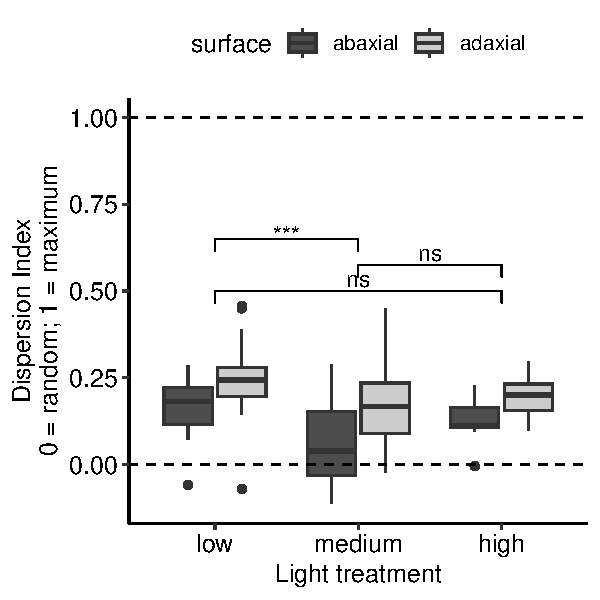
\includegraphics[width=\textwidth]{figures/single-surface.pdf}
\caption{Stomata are more dispersed than expected under the null model of uniform random position (dispersion index = 0) but far from a distribution that maximizes distance between stomata (dispersion index = 1). We determined statistical significance between light treatments using Tukey post-hoc tests. $^*~0.05 > P \ge 0.01; ^{**}~0.01 > P \ge 0.001; ^{***}~0.0001 > P \ge 0.0001; ^{***}~ P <0.0001$.}
\label{fig:single-surface}
\end{figure}

\hypertarget{no-evidence-for-coordinated-stomatal-position-between-surfaces}{%
\subsection{No evidence for coordinated stomatal position between
surfaces}\label{no-evidence-for-coordinated-stomatal-position-between-surfaces}}

There is no evidence of spatial coordination between abaxial and adaxial
leaf surfaces. The pixel-wise correlation between nearest stomatal
distance (NSD) squared on paired abaxial and adaxial leaf surfaces is
not significantly less than zero in any of the 66 leaves
(\autoref{fig:dual-surface}). Before controlling for multiple
comparisons, 3\% are significantly \emph{positively} correlated. The NSD
correlation is not different among light treatments (ANOVA,
\(F_{2,63} = 2.28, P = 0.111\); \autoref{fig:dual-surface}).

\begin{figure}[ht]
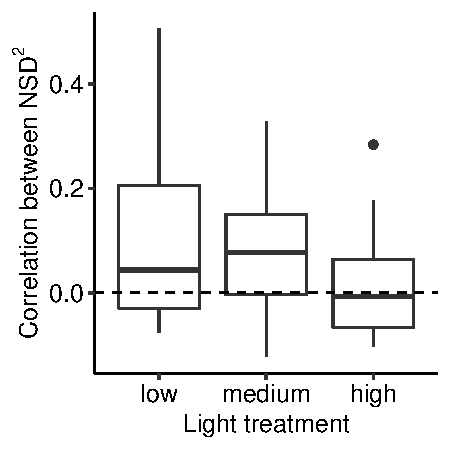
\includegraphics[width = \textwidth]{figures/dual-surface.pdf}
\caption{Correlation between paired abaxial and adaxial leaf surfaces. Dashed line indicates no correlation. Weak positive correlations are not significantly different from null simulations. No differences in abaxial-adaxial correlation were observed between light levels according to an analysis of variance ($\alpha$ = 0.05).}
\label{fig:dual-surface}
\end{figure}

Across all light treatments and leaf surfaces, stomatal length and
stomatal area were weakly positively correlated, indicating some support
for our hypothesis that stomata are selected for an optimal operational
aperture (\autoref{fig:length-area}).

\begin{figure}[ht]
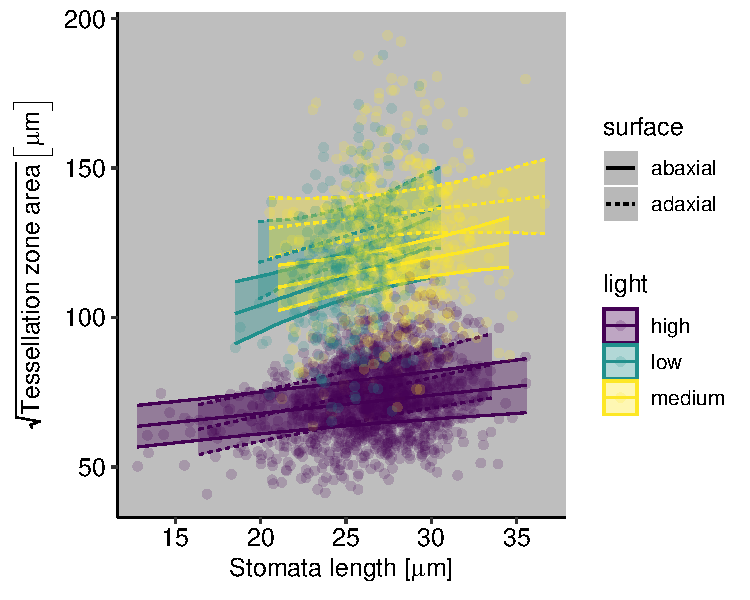
\includegraphics[width = \textwidth]{figures/length-area.pdf}
\caption{Stomatal length and stomatal zone area. Lines of best fit computed using a bayesian generalized non-linear multilevel model. Each light level and leaf surface exhibits a unique, weakly positive relationship between stomatal zone area and length.}
\label{fig:length-area}
\end{figure}

\hypertarget{discussion}{%
\section{Discussion}\label{discussion}}

Stomata are expensive. A theoretical, optimized plant would minimize
stomatal density while also allowing competitive gas exchange rates for
its environment so as to maximize C assimilation per unit investment in
stomata. Natural selection operates within developmental and physical
constraints to drive each plant species toward its theoretical optimum.
This study provides evidence that stomata in \emph{Arbidopsis thaliana},
the model angiosperm, are non-randomly distributed, favoring dispersion
over clustering (\autoref{fig:single-surface}). However, stomata are not
ideally dispersed in an equilateral triangular grid as would be optimal
to minimize CO\(_2\) diffusion path length and standardize the area
supplied by each stomate (\autoref{fig:tessellation-example}).
Additionally, when grown in high light environments, \emph{A. thaliana}
exhibited increased stomatal density rather than increased stomatal
dispersion (\autoref{fig:density}), which suggests that natural
selection has acted more strongly on developmental pathways that
modulate stomatal density than those that control stomatal dispersion.
In other words, plants optimize gas exchange by adding more stomata
rather than dispersing them more evenly across the leaf surface. This
study also demonstrates that stomata that supply larger leaf areas with
CO\(_2\) tend to be larger (\autoref{fig:length-area}). These results
could suggest that 1) the added energetic and hydraulic cost of
non-ideally dispersed stomata is negligible and therefore not acted on
by natural selection; 2) no developmental pathway exists to ensure the
ideal placement of stomata on the leaf; or 3) the regulation of stomatal
size limits the cost incurred by non-ideal stomatal dispersion.

In high light environments, amphistomy is favorable as high light
photosynthesis is limited by CO\(_2\) and amphistomy halves diffusion
path length and boundary layer resistance, thereby reducing CO\(_2\)
limitation - increasing theoretical \(A_\text{max}\). An optimal
amphistomatous leaf has offset stomata such that stomata are more likely
to appear on one leaf surface if there is not a stomata directly
opposite it on the other surface as shown in
\autoref{fig:ideal-amphi-grid}. However, our results show that leaf
surfaces are not coordinated but are independent, regardless of light
(\autoref{fig:dual-surface}). Additionally, gas exchange models show
little photosynthetic efficiency gain from abaxial-adaxial stomatal
coordination compared to anticoordination (INSERT FIG FROM MODELING). We
posit that this marginal gain is not sufficient to be acted upon
strongly by natural selection. Thus, amphistomatous plants do not
exhibit abaxial-adaxial stomatal coordination for there is little
selective advantage of it.

Our study corroborates previous studies which demonstrate that stomata
are non-randomly distributed along the leaf surface as a result of
developmental mechanisms such as spatially biased arrest of stomatal
initials (\protect\hyperlink{ref-boetsch_arrest_1995}{Boetsch, Chin, and
Croxdale 1995}), oriented asymmetric cell division
(\protect\hyperlink{ref-geisler_oriented_2000}{Geisler, Nadeau, and Sack
2000}), and cell cycle controls
(\protect\hyperlink{ref-croxdale_stomatal_2000}{Croxdale 2000}). We do
not investigate the potential developmental pathways that influence
stomatal dispersion in this study; however, they are important to
consider as these pathways could limit plants from reaching the
theoretical peak in the adaptive landscape: uniform stomatal dispersion.
Instead, as this study suggests, plants may simply compensate with
higher stomatal density and by fitting stomatal size to the area that
they supply with CO\(_2\). To understand why stomata are not ideally
dispersed, more modelling should be done to estimate the fitness gain of
stomatal dispersion. Additionally, genetic manipulation studies should
attempt to create mutants with clustered and ideally dispersed stomata
for a comparison of their photosynthetic traits. This could have
extremely important implications for maximum assimilation rates in crops
as most crop species are grown in high light where CO\(_2\) is often
limiting. In drought-prone environments, increased stomatal dispersion
may increase water use efficiency by reducing the number of stomata
needed to achieve the same internal CO\(_2\) concentration,
\(C_\text{i}\).

Beyond disperson on a single surface, gas exchange can be optimized via
stomatal coordination of abaxial and adaxial surfaces in amphistomatous
leaves. Given that leaf thicknesses are generally multiple times greater
than interstomatal distance (GIVE DISTANCES HERE). As a result,
abaxial-adaxial stomatal coordination reduces CO\(_2\) diffusion path
length far less than single surface dispersion, so we hypothesize this
strategy to afford less photosynthetic advantage to the leaf. Our
modelling results demonstrate that, even in ideal conditions, i.e.~thick
leaf, low stomatal densities, high light, low leaf porosity, high
Rubisco concentration, etc., the photosynthetic advantage of
coordination is minimal. We are not surprised by these results, but
still highlight them here as we are the first to report this finding.

Amphistomy is a unique and important adaptation found around the world
across many plant lineages
(\protect\hyperlink{ref-muir_light_2018}{Christopher D. Muir 2018}), yet
much of the dynamics of amphistomy remain poorly understood. Here, we
show that in \emph{Arabidopsis thaliana} 1) stomata in are non-randomly
dispersed, but not ideally dispersed; 2) stomatal size and density are
modulated by light; 3) stomatal size is positively correlated with the
area to which it supplies CO\(_2\); and 4) abaxial-adaxial stomatal
coordination is not exhibited and is not shown to provide a strong
photosynthetic advantage using CO\(_2\) diffusion models. Interestingly,
these findings did not validate many of our hypotheses which were based
on first principles, suggesting that there may be limits on plants'
ability to control stomatal placement. Future studies which elucidate
these limitations may have important implications for agriculturaly
productivity in a rapidly changing world.

\hypertarget{references}{%
\section*{References}\label{references}}
\addcontentsline{toc}{section}{References}

\hypertarget{refs}{}
\begin{CSLReferences}{1}{0}
\leavevmode\vadjust pre{\hypertarget{ref-aalto_three-dimensional_2002}{}}%
Aalto, T., and E. Juurola. 2002. {``A Three-Dimensional Model of {CO}
\(_{\textrm{2}}\) Transport in Airspaces and Mesophyll Cells of a Silver
Birch Leaf: {CO} \(_{\textrm{2}}\) Transport Inside a Birch Leaf.''}
\emph{Plant, Cell \& Environment} 25 (11): 1399--409.
\url{https://doi.org/10.1046/j.0016-8025.2002.00906.x}.

\leavevmode\vadjust pre{\hypertarget{ref-boetsch_arrest_1995}{}}%
Boetsch, John, Jonathan Chin, and Judith Croxdale. 1995. {``Arrest of
{Stomatal} {Initials} in {Tradescantia} {Is} {Linked} to the {Proximity}
of {Neighboring} {Stomata} and {Results} in the {Arrested} {Initials}
{Acquiring} {Properties} of {Epidermal} {Cells}.''} \emph{Developmental
Biology} 168 (1): 28--38. \url{https://doi.org/10.1006/dbio.1995.1058}.

\leavevmode\vadjust pre{\hypertarget{ref-buckley_optimal_2017}{}}%
Buckley, Thomas N, Lawren Sack, and Graham D Farquhar. 2017. {``Optimal
Plant Water Economy.''} \emph{Plant, Cell \& Environment} 40 (6):
881--96. \url{https://doi.org/10.1111/pce.12823}.

\leavevmode\vadjust pre{\hypertarget{ref-burkner_brms_2017}{}}%
Bürkner, Paul-Christian. 2017. {``\textbf{Brms} : {An} \emph{r}
{Package} for {Bayesian} {Multilevel} {Models} {Using} \emph{Stan}.''}
\emph{Journal of Statistical Software} 80 (1).
\url{https://doi.org/10.18637/jss.v080.i01}.

\leavevmode\vadjust pre{\hypertarget{ref-burkner_advanced_2018}{}}%
---------. 2018. {``Advanced {Bayesian} {Multilevel} {Modeling} with the
{R} {Package} Brms.''} \emph{The R Journal} 10 (1): 395.
\url{https://doi.org/10.32614/RJ-2018-017}.

\leavevmode\vadjust pre{\hypertarget{ref-bussis_stomatal_2006}{}}%
Büssis, Dirk, Uritza von Groll, Joachim Fisahn, and Thomas Altmann.
2006. {``Stomatal Aperture Can Compensate Altered Stomatal Density in
{Arabidopsis} Thaliana at Growth Light Conditions.''} \emph{Functional
Plant Biology} 33 (11): 1037. \url{https://doi.org/10.1071/FP06078}.

\leavevmode\vadjust pre{\hypertarget{ref-camargo_density_2011}{}}%
Camargo, Miguel Angelo Branco, and Ricardo Antonio Marenco. 2011.
{``Density, Size and Distribution of Stomata in 35 Rainforest Tree
Species in {Central} {Amazonia}.''} \emph{Acta Amazonica} 41 (2):
205--12. \url{https://doi.org/10.1590/S0044-59672011000200004}.

\leavevmode\vadjust pre{\hypertarget{ref-carriqui_diffusional_2015}{}}%
Carriquí, M., H. M. Cabrera, M. À. Conesa, R. E. Coopman, C. Douthe, J.
Gago, A. Gallé, et al. 2015. {``Diffusional Limitations Explain the
Lower Photosynthetic Capacity of Ferns as Compared with Angiosperms in a
Common Garden Study: {Photosynthetic} Comparison in Ferns and
Angiosperms.''} \emph{Plant, Cell \& Environment} 38 (3): 448--60.
\url{https://doi.org/10.1111/pce.12402}.

\leavevmode\vadjust pre{\hypertarget{ref-clark_distance_1954}{}}%
Clark, Philip J., and Francis C. Evans. 1954. {``Distance to Nearest
Neighbor as a Measure of Spatial Relationships in Populations.''}
\emph{Ecology} 35 (4): 445--53. \url{https://doi.org/10.2307/1931034}.

\leavevmode\vadjust pre{\hypertarget{ref-cowan_stomatal_1977}{}}%
Cowan, IR, and GD Farquhar. 1977. {``Stomatal Function in Relation to
Leaf Metabolism and Environment.''} \emph{STOMATAL FUNCTION IN RELATION
TO LEAF METABOLISM AND ENVIRONMENT.}

\leavevmode\vadjust pre{\hypertarget{ref-croxdale_stomatal_2000}{}}%
Croxdale, Judith L. 2000. {``Stomatal Patterning in Angiosperms.''}
\emph{American Journal of Botany} 87 (8): 1069--80.
\url{https://doi.org/10.2307/2656643}.

\leavevmode\vadjust pre{\hypertarget{ref-deans_optimization_2020}{}}%
Deans, Ross M., Timothy J. Brodribb, Florian A. Busch, and Graham D.
Farquhar. 2020. {``Optimization Can Provide the Fundamental Link Between
Leaf Photosynthesis, Gas Exchange and Water Relations.''} \emph{Nature
Plants} 6 (9): 1116--25.
\url{https://doi.org/10.1038/s41477-020-00760-6}.

\leavevmode\vadjust pre{\hypertarget{ref-dow_physiological_2014}{}}%
Dow, Graham J., Joseph A. Berry, and Dominique C. Bergmann. 2014. {``The
Physiological Importance of Developmental Mechanisms That Enforce Proper
Stomatal Spacing in \emph{{\textless{}}Span
Style="font-Variant:small-Caps;"{\textgreater{}}{A}{\textless{}}/Span{\textgreater{}}
Rabidopsis Thaliana}.''} \emph{New Phytologist} 201 (4): 1205--17.
\url{https://doi.org/10.1111/nph.12586}.

\leavevmode\vadjust pre{\hypertarget{ref-drake_two_2019}{}}%
Drake, Paul L., Hugo J. Boer, Stanislaus J. Schymanski, and Erik J.
Veneklaas. 2019. {``Two Sides to Every Leaf: Water and {\textless{}}Span
Style="font-Variant:small-Caps;"{\textgreater{}}{CO}{\textless{}}/Span{\textgreater{}}
\(_{\textrm{2}}\) Transport in Hypostomatous and Amphistomatous
Leaves.''} \emph{New Phytologist} 222 (3): 1179--87.
\url{https://doi.org/10.1111/nph.15652}.

\leavevmode\vadjust pre{\hypertarget{ref-earles_beyond_2018}{}}%
Earles, J. Mason, Guillaume Theroux-Rancourt, Adam B. Roddy, Matthew E.
Gilbert, Andrew J. McElrone, and Craig R. Brodersen. 2018. {``Beyond
{Porosity}: {3D} {Leaf} {Intercellular} {Airspace} {Traits} {That}
{Impact} {Mesophyll} {Conductance}.''} \emph{Plant Physiology} 178 (1):
148--62. \url{https://doi.org/10.1104/pp.18.00550}.

\leavevmode\vadjust pre{\hypertarget{ref-evans_resistances_2009}{}}%
Evans, J. R., R. Kaldenhoff, B. Genty, and I. Terashima. 2009.
{``Resistances Along the {CO}\(_{\textrm{2}}\) Diffusion Pathway Inside
Leaves.''} \emph{Journal of Experimental Botany} 60 (8): 2235--48.
\url{https://doi.org/10.1093/jxb/erp117}.

\leavevmode\vadjust pre{\hypertarget{ref-evans_spatialeco_2023}{}}%
Evans, Jeffrey S., and Melanie A. Murphy. 2023. \emph{{spatialEco}}.
\url{https://github.com/jeffreyevans/spatialEco}.

\leavevmode\vadjust pre{\hypertarget{ref-farquhar_biochemical_1980}{}}%
Farquhar, G. D., S. von Caemmerer, and J. A. Berry. 1980. {``A
Biochemical Model of Photosynthetic {CO2} Assimilation in Leaves of {C3}
Species.''} \emph{Planta} 149 (1): 78--90.
\url{https://doi.org/10.1007/BF00386231}.

\leavevmode\vadjust pre{\hypertarget{ref-franks_physiological_2012}{}}%
Franks, Peter J., Ilia J. Leitch, Elizabeth M. Ruszala, Alistair M.
Hetherington, and David J. Beerling. 2012. {``Physiological Framework
for Adaptation of Stomata to {CO} \(_{\textrm{2}}\) from Glacial to
Future Concentrations.''} \emph{Philosophical Transactions of the Royal
Society B: Biological Sciences} 367 (1588): 537--46.
\url{https://doi.org/10.1098/rstb.2011.0270}.

\leavevmode\vadjust pre{\hypertarget{ref-gay_influence_1975}{}}%
Gay, A. P., and R. G. Hurd. 1975. {``The Influence of Light on Stomatal
Density in the Tomato.''} \emph{New Phytologist} 75 (1): 37--46.
\url{https://doi.org/10.1111/j.1469-8137.1975.tb01368.x}.

\leavevmode\vadjust pre{\hypertarget{ref-geisler_oriented_2000}{}}%
Geisler, Matt, Jeanette Nadeau, and Fred D. Sack. 2000. {``Oriented
{Asymmetric} {Divisions} {That} {Generate} the {Stomatal} {Spacing}
{Pattern} in {Arabidopsis} {Are} {Disrupted} by the \emph{Too Many
Mouths} {Mutation}.''} \emph{The Plant Cell} 12 (11): 2075--86.
\url{https://doi.org/10.1105/tpc.12.11.2075}.

\leavevmode\vadjust pre{\hypertarget{ref-harrison_influence_2020}{}}%
Harrison, Emily L., Lucia Arce Cubas, Julie E. Gray, and Christopher
Hepworth. 2020. {``The Influence of Stomatal Morphology and Distribution
on Photosynthetic Gas Exchange.''} \emph{The Plant Journal} 101 (4):
768--79. \url{https://doi.org/10.1111/tpj.14560}.

\leavevmode\vadjust pre{\hypertarget{ref-harwood_understanding_2021}{}}%
Harwood, Richard, Guillaume Théroux‐Rancourt, and Margaret M Barbour.
2021. {``Understanding Airspace in Leaves: {\textless{}}Span
Style="font-Variant:small-Caps;"{\textgreater{}}{3D}{\textless{}}/Span{\textgreater{}}
Anatomy and Directional Tortuosity.''} \emph{Plant, Cell \&
Environment}, May, pce.14079. \url{https://doi.org/10.1111/pce.14079}.

\leavevmode\vadjust pre{\hypertarget{ref-jordan_using_2014}{}}%
Jordan, Gregory J., Raymond J. Carpenter, and Timothy J. Brodribb. 2014.
{``Using Fossil Leaves as Evidence for Open Vegetation.''}
\emph{Palaeogeography, Palaeoclimatology, Palaeoecology} 395 (February):
168--75. \url{https://doi.org/10.1016/j.palaeo.2013.12.035}.

\leavevmode\vadjust pre{\hypertarget{ref-jordan_environmental_2015}{}}%
Jordan, Gregory J., Raymond J. Carpenter, Anthony Koutoulis, Aina Price,
and Timothy J. Brodribb. 2015. {``Environmental Adaptation in Stomatal
Size Independent of the Effects of Genome Size.''} \emph{New
Phytologist} 205 (2): 608--17. \url{https://doi.org/10.1111/nph.13076}.

\leavevmode\vadjust pre{\hypertarget{ref-kaiser_metabolic_2016}{}}%
Kaiser, Elias, Alejandro Morales, Jeremy Harbinson, Ep Heuvelink, Aina
E. Prinzenberg, and Leo F. M. Marcelis. 2016. {``Metabolic and
Diffusional Limitations of Photosynthesis in Fluctuating Irradiance in
{Arabidopsis} Thaliana.''} \emph{Scientific Reports} 6 (1): 31252.
\url{https://doi.org/10.1038/srep31252}.

\leavevmode\vadjust pre{\hypertarget{ref-lange_responses_1971}{}}%
Lange, O. L., R. L�sch, E. -D. Schulze, and L. Kappen. 1971.
{``Responses of Stomata to Changes in Humidity.''} \emph{Planta} 100
(1): 76--86. \url{https://doi.org/10.1007/BF00386887}.

\leavevmode\vadjust pre{\hypertarget{ref-lee_diffusion_1964}{}}%
Lee, Richard, and David M. Gates. 1964. {``Diffusion Resistance in
Leaves as Related to Their Stomatal Anatomy and Micro-Structure.''}
\emph{American Journal of Botany} 51 (9): 963--75.
\url{https://doi.org/10.1002/j.1537-2197.1964.tb06725.x}.

\leavevmode\vadjust pre{\hypertarget{ref-lehmann_effects_2015}{}}%
Lehmann, Peter, and Dani Or. 2015. {``Effects of Stomata Clustering on
Leaf Gas Exchange.''} \emph{New Phytologist} 207 (4): 1015--25.
\url{https://doi.org/10.1111/nph.13442}.

\leavevmode\vadjust pre{\hypertarget{ref-lehmeier_cell_2017}{}}%
Lehmeier, Christoph, Radoslaw Pajor, Marjorie R. Lundgren, Andrew
Mathers, Jen Sloan, Marion Bauch, Alice Mitchell, et al. 2017. {``Cell
Density and Airspace Patterning in the Leaf Can Be Manipulated to
Increase Leaf Photosynthetic Capacity.''} \emph{The Plant Journal} 92
(6): 981--94. \url{https://doi.org/10.1111/tpj.13727}.

\leavevmode\vadjust pre{\hypertarget{ref-liu_scaling_2021}{}}%
Liu, Congcong, Christopher D. Muir, Ying Li, Li Xu, Mingxu Li, Jiahui
Zhang, Hugo Jan de Boer, et al. 2021. {``Scaling Between Stomatal Size
and Density in Forest Plants.''} Preprint. Plant Biology.
\url{https://doi.org/10.1101/2021.04.25.441252}.

\leavevmode\vadjust pre{\hypertarget{ref-manter_ci_2004}{}}%
Manter, D. K. 2004. {``A/{Ci} Curve Analysis Across a Range of Woody
Plant Species: Influence of Regression Analysis Parameters and Mesophyll
Conductance.''} \emph{Journal of Experimental Botany} 55 (408):
2581--88. \url{https://doi.org/10.1093/jxb/erh260}.

\leavevmode\vadjust pre{\hypertarget{ref-mcadam_linking_2016}{}}%
McAdam, Scott A. M., and Timothy J. Brodribb. 2016. {``Linking {Turgor}
with {ABA} {Biosynthesis}: {Implications} for {Stomatal} {Responses} to
{Vapor} {Pressure} {Deficit} Across {Land} {Plants}.''} \emph{Plant
Physiology} 171 (3): 2008--16.
\url{https://doi.org/10.1104/pp.16.00380}.

\leavevmode\vadjust pre{\hypertarget{ref-morison_lateral_2005}{}}%
Morison, James I. L., Emily Gallouët, Tracy Lawson, Gabriel Cornic,
Raphaèle Herbin, and Neil R. Baker. 2005. {``Lateral {Diffusion} of {CO}
{\textless{}}Sub{\textgreater{}}2{\textless{}}sub{\textgreater{}} in
{Leaves} {Is} {Not} {Sufficient} to {Support} {Photosynthesis}.''}
\emph{Plant Physiology} 139 (1): 254--66.
\url{https://doi.org/10.1104/pp.105.062950}.

\leavevmode\vadjust pre{\hypertarget{ref-mott_adaptive_1982}{}}%
Mott, Keith A., Arthur C. Gibson, and James W. O'Leary. 1982. {``The
Adaptive Significance of Amphistomatic Leaves.''} \emph{Plant, Cell \&
Environment} 5 (6): 455--60.
\url{https://doi.org/10.1111/1365-3040.ep11611750}.

\leavevmode\vadjust pre{\hypertarget{ref-mott_amphistomy_1991}{}}%
Mott, Keith A., and Odette Michaelson. 1991. {``{AMPHISTOMY} {AS} {AN}
{ADAPTATION} {TO} {HIGH} {LIGHT} {INTENSITY} {IN} {AMBROSIA}
{CORDIFOLIA} ({COMPOSITAE}).''} \emph{American Journal of Botany} 78
(1): 76--79. \url{https://doi.org/10.1002/j.1537-2197.1991.tb12573.x}.

\leavevmode\vadjust pre{\hypertarget{ref-muir_is_2019}{}}%
Muir, Christopher D. 2019. {``Is {Amphistomy} an {Adaptation} to {High}
{Light}? {Optimality} {Models} of {Stomatal} {Traits} Along {Light}
{Gradients}.''} \emph{Integrative and Comparative Biology} 59 (3):
571--84. \url{https://doi.org/10.1093/icb/icz085}.

\leavevmode\vadjust pre{\hypertarget{ref-muir_light_2018}{}}%
Muir, Christopher D. 2018. {``Light and Growth Form Interact to Shape
Stomatal Ratio Among {British} Angiosperms.''} \emph{New Phytologist}
218 (1): 242--52. \url{https://doi.org/10.1111/nph.14956}.

\leavevmode\vadjust pre{\hypertarget{ref-muir_how_2023}{}}%
Muir, Christopher D., Miquel Àngel Conesa, Jeroni Galmés, Varsha S.
Pathare, Patricia Rivera, Rosana López Rodríguez, Teresa Terrazas, and
Dongliang Xiong. 2023. {``How Important Are Functional and Developmental
Constraints on Phenotypic Evolution? {An} Empirical Test with the
Stomatal Anatomy of Flowering Plants.''} \emph{The American Naturalist}
201 (6): 794--812. \url{https://doi.org/10.1086/723780}.

\leavevmode\vadjust pre{\hypertarget{ref-murray_consistent_2020}{}}%
Murray, Michelle, Wuu Kuang Soh, Charilaos Yiotis, Robert A. Spicer,
Tracy Lawson, and Jennifer C. McElwain. 2020. {``Consistent Relationship
Between Field-Measured Stomatal Conductance and Theoretical Maximum
Stomatal Conductance in {C}\(_{\textrm{3}}\) Woody Angiosperms in Four
Major Biomes.''} \emph{International Journal of Plant Sciences} 181 (1):
142--54. \url{https://doi.org/10.1086/706260}.

\leavevmode\vadjust pre{\hypertarget{ref-papanatsiou_stomatal_2017}{}}%
Papanatsiou, Maria, Anna Amtmann, and Michael R. Blatt. 2017.
{``Stomatal Clustering in {Begonia} Associates with the Kinetics of Leaf
Gaseous Exchange and Influences Water Use Efficiency.''} \emph{Journal
of Experimental Botany} 68 (9): 2309--15.
\url{https://doi.org/10.1093/jxb/erx072}.

\leavevmode\vadjust pre{\hypertarget{ref-parkhurst_adaptive_1978}{}}%
Parkhurst, David F. 1978. {``The {Adaptive} {Significance} of {Stomatal}
{Occurrence} on {One} or {Both} {Surfaces} of {Leaves}.''} \emph{Journal
of Ecology} 66 (2): 367--83. \url{https://doi.org/10.2307/2259142}.

\leavevmode\vadjust pre{\hypertarget{ref-parkhurst_diffusion_1994}{}}%
---------. 1994. {``Diffusion of {CO}\(_{\textrm{2}}\) and Other Gases
Inside Leaves.''} \emph{New Phytologist} 126 (3): 449--79.
\url{http://www.jstor.org/stable/2557929}.

\leavevmode\vadjust pre{\hypertarget{ref-parkhurst_intercellular_1990}{}}%
Parkhurst, David F., and Keith A. Mott. 1990. {``Intercellular
{Diffusion} {Limits} to {CO} \(_{\textrm{2}}\) {Uptake} in {Leaves}:
{Studies} in {Air} and {Helox}.''} \emph{Plant Physiology} 94 (3):
1024--32. \url{https://doi.org/10.1104/pp.94.3.1024}.

\leavevmode\vadjust pre{\hypertarget{ref-pieruschka_lateral_2005}{}}%
Pieruschka, R. 2005. {``Lateral Gas Diffusion Inside Leaves.''}
\emph{Journal of Experimental Botany} 56 (413): 857--64.
\url{https://doi.org/10.1093/jxb/eri072}.

\leavevmode\vadjust pre{\hypertarget{ref-pieruschka_lateral_2006}{}}%
Pieruschka, Roland, Ulrich Schurr, Manfred Jensen, Wilfried F. Wolff,
and Siegfried Jahnke. 2006. {``Lateral Diffusion of {CO}
\(_{\textrm{2}}\) from Shaded to Illuminated Leaf Parts Affects
Photosynthesis Inside Homobaric Leaves.''} \emph{New Phytologist} 169
(4): 779--88. \url{https://doi.org/10.1111/j.1469-8137.2005.01605.x}.

\leavevmode\vadjust pre{\hypertarget{ref-roddy_scaling_2020}{}}%
Roddy, Adam B., Guillaume Théroux-Rancourt, Tito Abbo, Joseph W.
Benedetti, Craig R. Brodersen, Mariana Castro, Silvia Castro, et al.
2020. {``The {Scaling} of {Genome} {Size} and {Cell} {Size} {Limits}
{Maximum} {Rates} of {Photosynthesis} with {Implications} for
{Ecological} {Strategies}.''} \emph{International Journal of Plant
Sciences} 181 (1): 75--87. \url{https://doi.org/10.1086/706186}.

\leavevmode\vadjust pre{\hypertarget{ref-royer_stomatal_2001}{}}%
Royer, D. L. 2001. {``Stomatal Density and Stomatal Index as Indicators
of Paleoatmospheric {CO2} Concentration.''} \emph{Review of Palaeobotany
and Palynology} 114 (1-2): 1--28.
\url{https://doi.org/10.1016/S0034-6667(00)00074-9}.

\leavevmode\vadjust pre{\hypertarget{ref-sachs_developmental_1974}{}}%
Sachs, T. 1974. {``The {Developmental} {Origin} of {Stomata} {Pattern}
in {Crinum}.''} \emph{Botanical Gazette} 135 (4): 314--18.
\url{https://doi.org/10.1086/336767}.

\leavevmode\vadjust pre{\hypertarget{ref-sack_developmental_2016}{}}%
Sack, Lawren, and Thomas N. Buckley. 2016. {``The {Developmental}
{Basis} of {Stomatal} {Density} and {Flux}.''} \emph{Plant Physiology}
171 (4): 2358--63. \url{https://doi.org/10.1104/pp.16.00476}.

\leavevmode\vadjust pre{\hypertarget{ref-schneider_nih_2012}{}}%
Schneider, Caroline A, Wayne S Rasband, and Kevin W Eliceiri. 2012.
{``{NIH} {Image} to {ImageJ}: 25 Years of Image Analysis.''}
\emph{Nature Methods} 9 (7): 671--75.
\url{https://doi.org/10.1038/nmeth.2089}.

\leavevmode\vadjust pre{\hypertarget{ref-schoch_dependence_1980}{}}%
Schoch, Paul-G., Claude Zinsou, and Monique Sibi. 1980. {``Dependence of
the {Stomatal} {Index} on {Environmental} {Factors} During {Stomatal}
{Differentiation} in {Leaves} of \emph{{Vigna} Sinensis} {L}.: 1.
{EFFECT} {OF} {LIGHT} {INTENSITY}.''} \emph{Journal of Experimental
Botany} 31 (5): 1211--16. \url{https://doi.org/10.1093/jxb/31.5.1211}.

\leavevmode\vadjust pre{\hypertarget{ref-sperry_predicting_2017}{}}%
Sperry, John S., Martin D. Venturas, William R. L. Anderegg, Maurizio
Mencuccini, D. Scott Mackay, Yujie Wang, and David M. Love. 2017.
{``Predicting Stomatal Responses to the Environment from the
Optimization of Photosynthetic Gain and Hydraulic Cost: {A} Stomatal
Optimization Model.''} \emph{Plant, Cell \& Environment} 40 (6):
816--30. \url{https://doi.org/10.1111/pce.12852}.

\leavevmode\vadjust pre{\hypertarget{ref-woodward_stomatal_1987}{}}%
Woodward, F. I. 1987. {``Stomatal Numbers Are Sensitive to Increases in
{CO2} from Pre-Industrial Levels.''} \emph{Nature} 327 (6123): 617--18.
\url{https://doi.org/10.1038/327617a0}.

\leavevmode\vadjust pre{\hypertarget{ref-yi_gan_stomatal_2010}{}}%
Yi Gan, Lei Zhou, Zhong-Ji Shen, Zhu-Xia Shen, Yi-Qiong Zhang, and
Gen-Xuan Wang. 2010. {``Stomatal Clustering, a New Marker for
Environmental Perception and Adaptation in Terrestrial Plants.''}
\emph{Botanical Studies} 51 (3): 325--36.
\url{https://search.ebscohost.com/login.aspx?direct=true\&db=a9h\&AN=60102322\&site=ehost-live}.

\end{CSLReferences}


\begin{notes}[Acknowledgements]
This is an acknowledgement.

It consists of two paragraphs.
\end{notes}




\end{document}
